\documentclass[border=10pt]{standalone}
\usepackage[svgnames]{xcolor}
\usepackage{amsmath}
\usepackage{pgfplots}
\pgfplotsset{compat=newest}
\usepackage[sfdefault]{FiraSans}
\usepackage{FiraMono}
\renewcommand*\familydefault{\sfdefault}
\begin{document}
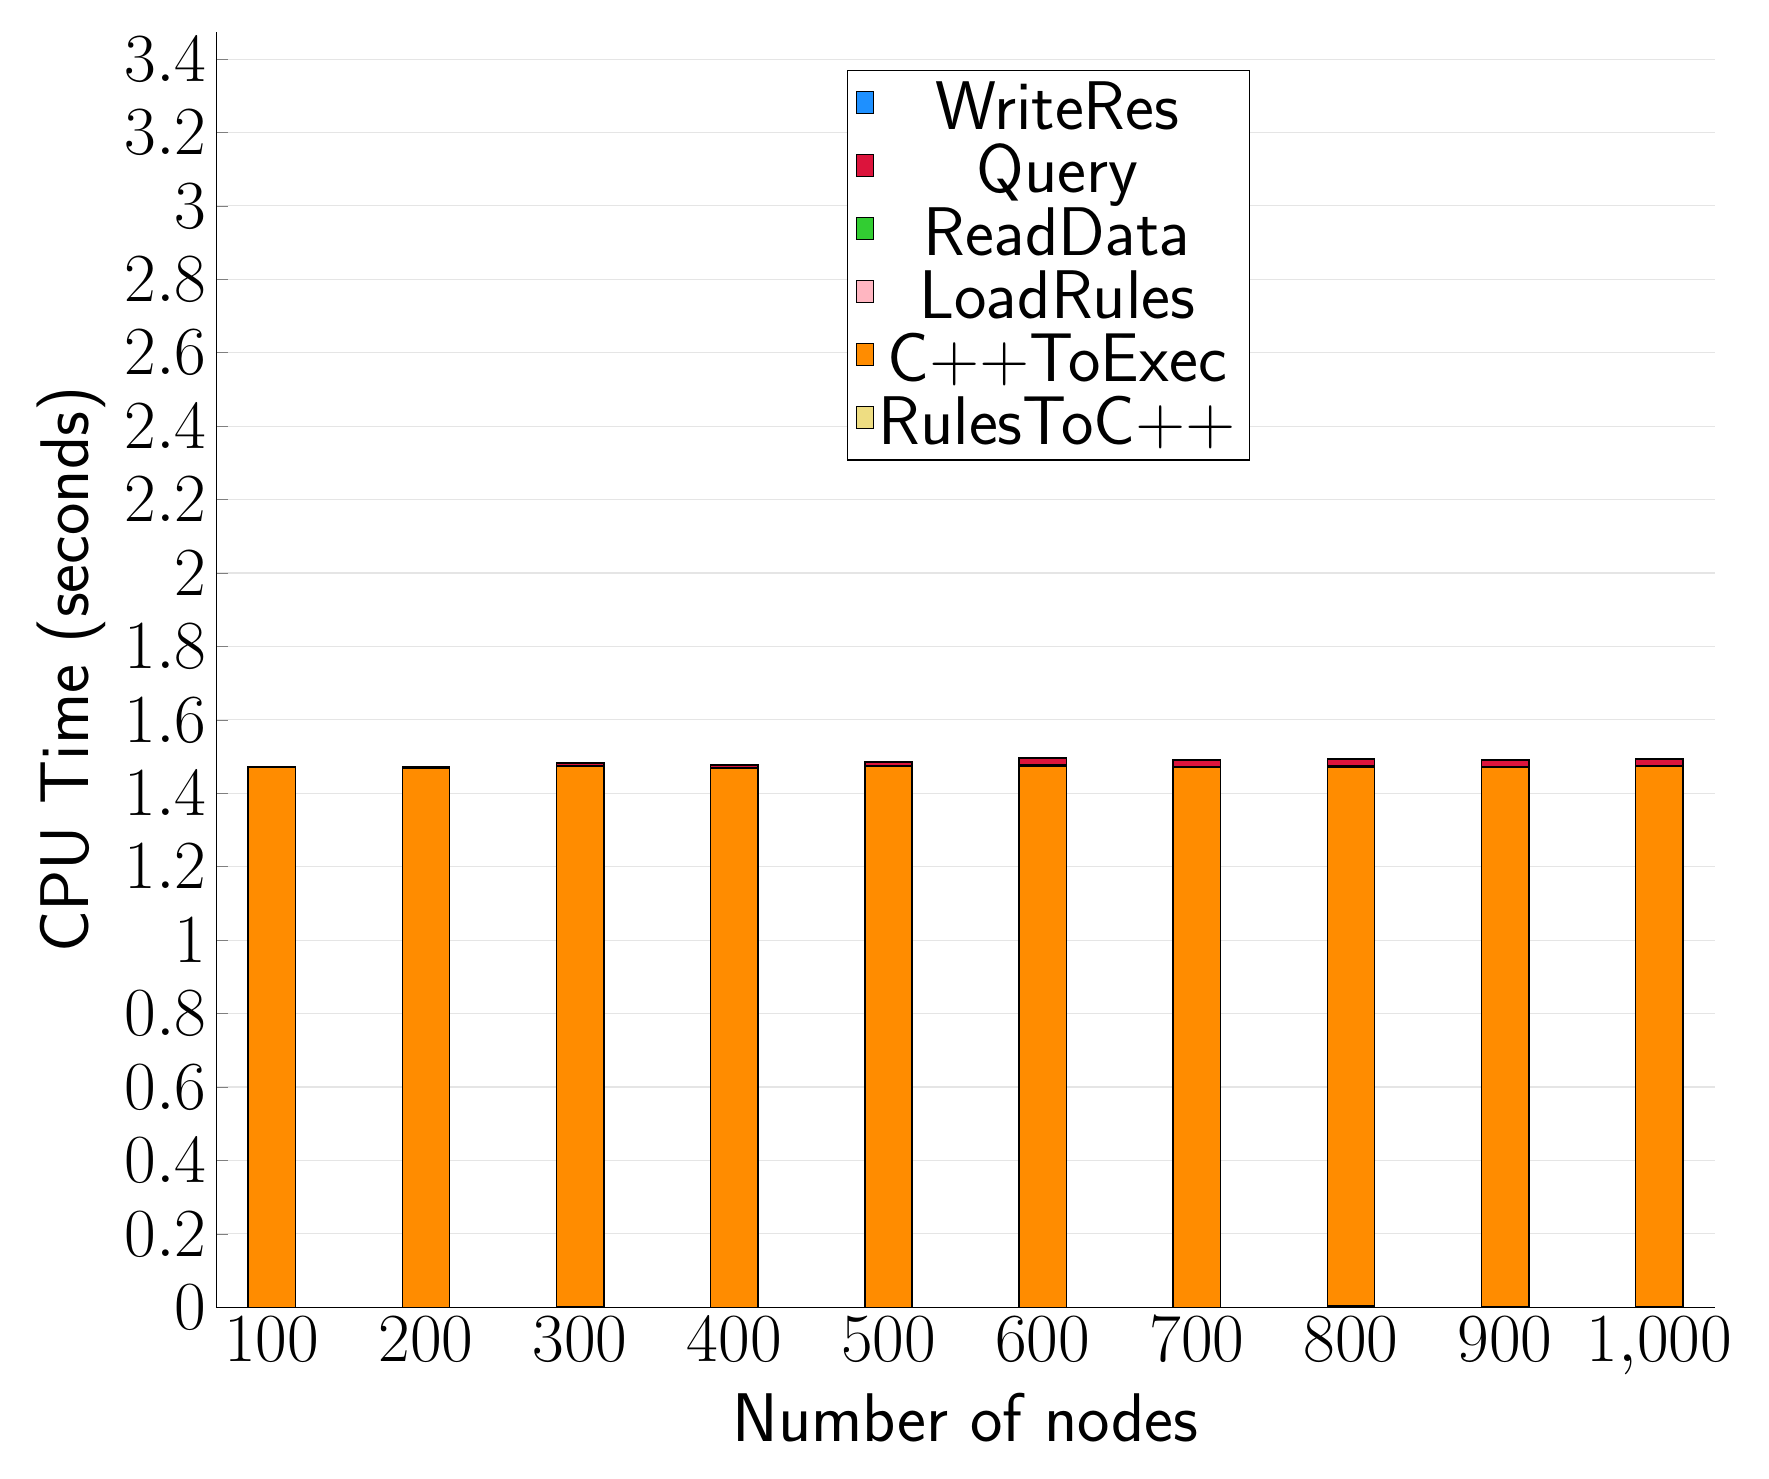
\begin{tikzpicture}
\begin{axis}[
   ybar stacked,
   width=1.7\textwidth,
   bar width=0.6cm,
   ymajorgrids, tick align=inside,
   major grid style={draw=gray!20},
   xtick=data,
   ymin=0, ymax=3.4739999999999998,
   axis x line*=bottom,
   axis y line*=left,
   enlarge x limits=0.04,
   legend style={
       at={(0.69, 0.97)},
       anchor=north east,
       legend columns=1,
       font=\Huge,
   },
   ylabel={CPU Time (seconds)},
   xlabel={Number of nodes},
   label style={font=\Huge},
   tick label style={font=\Huge},
]
\addlegendimage{fill=DodgerBlue, draw=black, line width=0.2pt}
\addlegendentry{WriteRes}
\addlegendimage{fill=Crimson, draw=black, line width=0.2pt}
\addlegendentry{Query}
\addlegendimage{fill=LimeGreen, draw=black, line width=0.2pt}
\addlegendentry{ReadData}
\addlegendimage{fill=LightPink, draw=black, line width=0.2pt}
\addlegendentry{LoadRules}
\addlegendimage{fill=DarkOrange, draw=black, line width=0.2pt}
\addlegendentry{C++ToExec}
\addlegendimage{fill=LightGoldenrod, draw=black, line width=0.2pt}
\addlegendentry{RulesToC++}
\addplot +[fill=LightGoldenrod, draw=black, line width=0.55pt] coordinates {
(100, 0.0)
(200, 0.0)
(300, 0.0020000000000000005)
(400, 0.0)
(500, 0.0)
(600, 0.0)
(700, 0.0)
(800, 0.004000000000000001)
(900, 0.0020000000000000005)
(1000, 0.0020000000000000005)
};
\addplot +[fill=DarkOrange, draw=black, line width=0.55pt] coordinates {
(100, 1.47)
(200, 1.468)
(300, 1.472)
(400, 1.468)
(500, 1.4739999999999998)
(600, 1.4739999999999998)
(700, 1.47)
(800, 1.468)
(900, 1.4679999999999997)
(1000, 1.472)
};
\addplot +[fill=LightPink, draw=black, line width=0.55pt] coordinates {
(100, 0.0001902)
(200, 0.0001756)
(300, 0.0001814)
(400, 0.0001796)
(500, 0.000182)
(600, 0.0001882)
(700, 0.00017900000000000001)
(800, 0.0001848)
(900, 0.0001828)
(1000, 0.0001778)
};
\addplot +[fill=LimeGreen, draw=black, line width=0.55pt] coordinates {
(100, 0.0006564)
(200, 0.000898)
(300, 0.0011886)
(400, 0.0013072000000000001)
(500, 0.001416)
(600, 0.0022876)
(700, 0.00237)
(800, 0.0022834)
(900, 0.0023404000000000003)
(1000, 0.0021686)
};
\addplot +[fill=Crimson, draw=black, line width=0.55pt] coordinates {
(100, 0.001444)
(200, 0.0035091999999999996)
(300, 0.0077176)
(400, 0.007373)
(500, 0.008685)
(600, 0.0179876)
(700, 0.017821999999999998)
(800, 0.017591600000000002)
(900, 0.0180928)
(1000, 0.017100800000000003)
};
\addplot +[fill=DodgerBlue, draw=black, line width=0.55pt] coordinates {
(100, 0.0006638)
(200, 0.0008238000000000001)
(300, 0.0010945999999999998)
(400, 0.0010462000000000002)
(500, 0.0010773999999999998)
(600, 0.0018882)
(700, 0.0018633999999999999)
(800, 0.0018478000000000001)
(900, 0.0018590000000000002)
(1000, 0.001808)
};
\end{axis}
\end{tikzpicture}

\end{document}
